\documentclass[10pt]{article}
\usepackage[a4paper,margin=18mm]{geometry}
\usepackage{amsmath,amssymb,booktabs,array,enumitem}
\usepackage[T1]{fontenc}\usepackage{lmodern}
\usepackage{tikz}\usetikzlibrary{shapes.gates.logic.US,positioning,arrows.meta,calc}
\usepackage[hidelinks]{hyperref}
\setlength{\parindent}{0pt}\setlength{\parskip}{4pt}\setlength{\emergencystretch}{2em}
\newcommand{\VDD}{V_{DD}}
\newcommand{\mos}[4]{\begin{scope}[shift={(#1,#2)}]
\draw(0,.23)--(0,-.23);\draw(0,.2)--(.25,.2)--(.25,.5);\draw(0,-.2)--(.25,-.2)--(.25,-.5);
\draw(-.16,.23)--(-.16,-.23);
\ifnum#4=1\draw(-.26,0)circle(.06);\draw(-.7,0)--(-.32,0);\else\draw(-.7,0)--(-.16,0);\fi
\node[anchor=east,font=\scriptsize]at(-.71,0){$#3$};\end{scope}}
\newcommand{\grd}[2]{\draw(#1,#2)--(#1,#2-.12);\draw(#1-.15,#2-.12)--(#1+.15,#2-.12);\draw(#1-.1,#2-.19)--(#1+.1,#2-.19);}
\newcommand{\rail}[3]{\draw(#1,#2)--(#1,#2+.2)node[above]{$#3$};}
\begin{document}\begin{center}{\large\bfseries EE3032 Introduction to VLSI -- Midterm}\end{center}
\textbf{Fall 2009.} All six original questions; printed points sum to 105.
\textbf{1. (30 points)} Answer the following problems.
\begin{enumerate}[label=(\alph*),leftmargin=7mm,itemsep=1pt]
\item Explain the purpose of design rules in VLSI design. (4 points)
\item Realize the Boolean function $f=\overline{x_1+x_2x_3+x_4}$ with static CMOS logic. (4 points)
\item What is antenna effect? (3 points)
\item List four properties of static CMOS logic. (4 points)
\item Explain why adding a guard ring can reduce the latchup effect. (4 points)
\item List two possible approaches for alleviating the effect of crosstalk on two neighboring parallel interconnects. (4 points)
\item Explain the energy consumption of an inverter when the inverter performs a switching. (4 points)
\item List the three major components of the load capacitance of a CMOS logic gate in a CMOS circuit. (3 points)
\end{enumerate}
\textbf{2. (10 points)} Figure 1 depicts the process cross section of a CMOS inverter.
\begin{enumerate}[label=(\alph*),leftmargin=7mm]
\item Draw the circuit-level model for modeling the latchup phenomenon. (5 points)
\item Explain the phenomenon of latchup based on the model derived in (a). (5 points)
\end{enumerate}
\begin{center}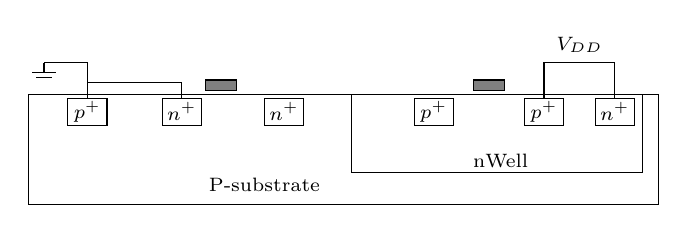
\begin{tikzpicture}[x=1cm,y=1cm,font=\scriptsize]
\draw(0,0)rectangle(8,1.4);\draw(4.1,.4)rectangle(7.8,1.4);\node at(6,.55){nWell};\node at(3,.25){P-substrate};
\foreach\x/\t in{.5/p^+,1.7/n^+,3/n^+,4.9/p^+,6.3/p^+,7.2/n^+}{\draw(\x,1)rectangle(\x+.5,1.35);\node at(\x+.25,1.18){$\t$};}
\foreach\x in{2.45,5.85}{\draw[fill=gray](\x-.2,1.45)rectangle(\x+.2,1.58);}
\draw(.75,1.35)--(.75,1.55)--(1.95,1.55)--(1.95,1.35);\draw(.75,1.55)--(.75,1.8)--(.2,1.8);\grd{.2}{1.8}
\draw(6.55,1.35)--(6.55,1.8)--(7.45,1.8)--(7.45,1.35);\node[above]at(7,1.8){$V_{DD}$};
\end{tikzpicture}\\Figure 1: Process cross section of a CMOS inverter.\end{center}
\textbf{3. (10 points)} Figure 2 depicts two designs of inverter chains. Assume that the equivalent resistance of a minimum size W/L NMOS is $R$ and $\mu_n=2\mu_p$. The gate capacitance of a W/L transistor is $C_g$. Also, the parasitic capacitance of drain/source and wires are neglected. Which inverter chain consumes lower short-circuit power? Explain your answer.
\begin{center}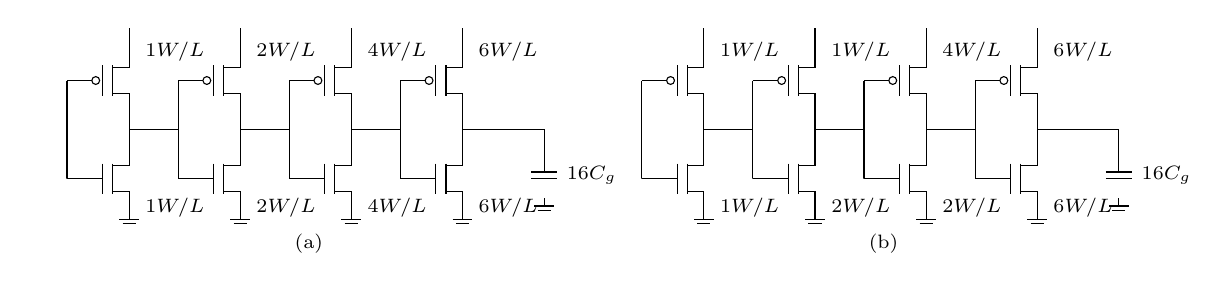
\begin{tikzpicture}[x=.83cm,y=.83cm,font=\scriptsize]\begin{scope}[xshift=0cm]
\mos{0.0}{2.5}{\phantom{X}}{1}\mos{0.0}{1}{\phantom{X}}{0}
\draw(0.25,3)--(0.25,3.3);\draw(0.25,2)--(0.25,1.5);\grd{0.25}{.5}
\draw(-0.7,2.5)--(-0.7,1)--(-0.7,1.75);
\node[above right]at(0.35,2.65){$1W/L$};\node[below right]at(0.35,.85){$1W/L$};
\draw(0.25,1.75)--(1.0,1.75);
\mos{1.7}{2.5}{\phantom{X}}{1}\mos{1.7}{1}{\phantom{X}}{0}
\draw(1.95,3)--(1.95,3.3);\draw(1.95,2)--(1.95,1.5);\grd{1.95}{.5}
\draw(1.0,2.5)--(1.0,1)--(1.0,1.75);
\node[above right]at(2.05,2.65){$2W/L$};\node[below right]at(2.05,.85){$2W/L$};
\draw(1.95,1.75)--(2.7,1.75);
\mos{3.4}{2.5}{\phantom{X}}{1}\mos{3.4}{1}{\phantom{X}}{0}
\draw(3.65,3)--(3.65,3.3);\draw(3.65,2)--(3.65,1.5);\grd{3.65}{.5}
\draw(2.7,2.5)--(2.7,1)--(2.7,1.75);
\node[above right]at(3.75,2.65){$4W/L$};\node[below right]at(3.75,.85){$4W/L$};
\draw(3.65,1.75)--(4.4,1.75);
\mos{5.1}{2.5}{\phantom{X}}{1}\mos{5.1}{1}{\phantom{X}}{0}
\draw(5.35,3)--(5.35,3.3);\draw(5.35,2)--(5.35,1.5);\grd{5.35}{.5}
\draw(4.3999999999999995,2.5)--(4.3999999999999995,1)--(4.3999999999999995,1.75);
\node[above right]at(5.449999999999999,2.65){$6W/L$};\node[below right]at(5.449999999999999,.85){$6W/L$};
\draw(5.35,1.75)--(6.6,1.75)--(6.6,1.1);\draw(6.4,1.1)--(6.8,1.1) (6.4,1)--(6.8,1);\grd{6.6}{.7}\node[right]at(6.8,1.05){$16C_g$};
\node at(3,0){(a)};
\end{scope}\begin{scope}[xshift=7.3cm]
\mos{0.0}{2.5}{\phantom{X}}{1}\mos{0.0}{1}{\phantom{X}}{0}
\draw(0.25,3)--(0.25,3.3);\draw(0.25,2)--(0.25,1.5);\grd{0.25}{.5}
\draw(-0.7,2.5)--(-0.7,1)--(-0.7,1.75);
\node[above right]at(0.35,2.65){$1W/L$};\node[below right]at(0.35,.85){$1W/L$};
\draw(0.25,1.75)--(1.0,1.75);
\mos{1.7}{2.5}{\phantom{X}}{1}\mos{1.7}{1}{\phantom{X}}{0}
\draw(1.95,3)--(1.95,3.3);\draw(1.95,2)--(1.95,1.5);\grd{1.95}{.5}
\draw(1.0,2.5)--(1.0,1)--(1.0,1.75);
\node[above right]at(2.05,2.65){$1W/L$};\node[below right]at(2.05,.85){$2W/L$};
\draw(1.95,1.75)--(2.7,1.75);
\mos{3.4}{2.5}{\phantom{X}}{1}\mos{3.4}{1}{\phantom{X}}{0}
\draw(3.65,3)--(3.65,3.3);\draw(3.65,2)--(3.65,1.5);\grd{3.65}{.5}
\draw(2.7,2.5)--(2.7,1)--(2.7,1.75);
\node[above right]at(3.75,2.65){$4W/L$};\node[below right]at(3.75,.85){$2W/L$};
\draw(3.65,1.75)--(4.4,1.75);
\mos{5.1}{2.5}{\phantom{X}}{1}\mos{5.1}{1}{\phantom{X}}{0}
\draw(5.35,3)--(5.35,3.3);\draw(5.35,2)--(5.35,1.5);\grd{5.35}{.5}
\draw(4.3999999999999995,2.5)--(4.3999999999999995,1)--(4.3999999999999995,1.75);
\node[above right]at(5.449999999999999,2.65){$6W/L$};\node[below right]at(5.449999999999999,.85){$6W/L$};
\draw(5.35,1.75)--(6.6,1.75)--(6.6,1.1);\draw(6.4,1.1)--(6.8,1.1) (6.4,1)--(6.8,1);\grd{6.6}{.7}\node[right]at(6.8,1.05){$16C_g$};
\node at(3,0){(b)};
\end{scope}\end{tikzpicture}\end{center}\begin{center}Figure 2: Inverter chains.\end{center}
\newpage
\textbf{4. (30 points)} Figure 3(a) depicts a CMOS logic circuit. Assume that the delay of an inverter is one delay unit, where the inverter size is $W_p/L_p=2\,\mu m/.18\,\mu m$ and $W_n/L_n=1\,\mu m/.18\,\mu m$, and the input capacitance of the inverter is $C_i$. Also, assume that the size of each NMOS transistor and PMOS transistor of all the gates is the same as that of the inverter. When the CMOS logic circuit is operated, possible functional inputs of the circuit are $\{01001,11011,11100,01101\}$. Also, these inputs are applied in sequence and the frequency is $f$ and the power supply is $V_{DD}$.
\begin{enumerate}[label=(\alph*),leftmargin=7mm]
\item Estimate the peak power of this circuit in terms of $f,C_i,V_{DD}$. (10 points)
\item Determine the delay of each gate in terms of delay unit (neglect the diffusion and wire capacitance). (10 points)
\item Assume that a dual-$V_T$ process can be used to implement the CMOS circuit. Draw the transistor schematic diagram of the CMOS circuit in terms of the symbols shown in Figure 3(b) such that the leakage power of the CMOS circuit is minimal without sacrificing the speed of the CMOS circuit. (10 points)
\end{enumerate}
\begin{center}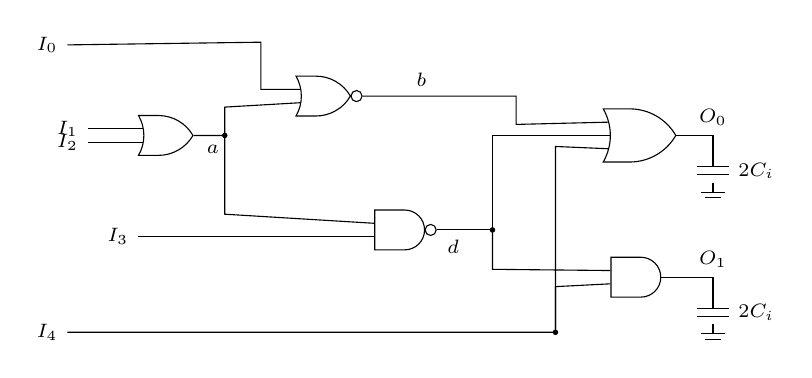
\begin{tikzpicture}[x=1cm,y=1cm,font=\scriptsize]
\node[or gate US,draw,logic gate inputs=nn](a)at(1,2){};
\node[nor gate US,draw,logic gate inputs=nn](b)at(3,2.5){};
\node[nand gate US,draw,logic gate inputs=nn](d)at(4,.8){};
\node[or gate US,draw,logic gate inputs=nnn](o0)at(7,2){};
\node[and gate US,draw,logic gate inputs=nn](o1)at(7,.2){};
\draw(a.input 1)--++(-.7,0)node[left]{$I_1$};\draw(a.input 2)--++(-.7,0)node[left]{$I_2$};
\draw(b.input 1)--++(-.5,0)--++(0,.6)--(-.2,3.15)node[left]{$I_0$};
\draw(a.output)--(1.8,2)coordinate(j)--(1.8,2.36)--(b.input 2);\fill(j)circle(1pt);\node[below]at(1.65,2){$a$};
\draw(j)--(1.8,1)--(d.input 1);\draw(d.input 2)--++(-3,0)node[left]{$I_3$};
\draw(b.output)--(5.5,2.5)--(5.5,2.14)--(o0.input 1);\node[above]at(4.3,2.5){$b$};
\draw(d.output)--(5.2,.8)coordinate(k)--(5.2,2)--(o0.input 2);\fill(k)circle(1pt);\node[below]at(4.7,.8){$d$};
\draw(k)--(5.2,.3)--(o1.input 1);\draw(-.2,-.5)node[left]{$I_4$}--(6,-.5)coordinate(l)--(6,.08)--(o1.input 2);
\draw(l)--(6,1.86)--(o0.input 3);\fill(l)circle(1pt);
\draw(o0.output)--(8,2)node[above]{$O_0$}--(8,1.6);\draw(7.8,1.6)--(8.2,1.6) (7.8,1.5)--(8.2,1.5);\grd{8}{1.4}\node[right]at(8.2,1.55){$2C_i$};
\draw(o1.output)--(8,.2)node[above]{$O_1$}--(8,-.2);\draw(7.8,-.2)--(8.2,-.2) (7.8,-.3)--(8.2,-.3);\grd{8}{-.4}\node[right]at(8.2,-.25){$2C_i$};
\end{tikzpicture}\end{center}\begin{center}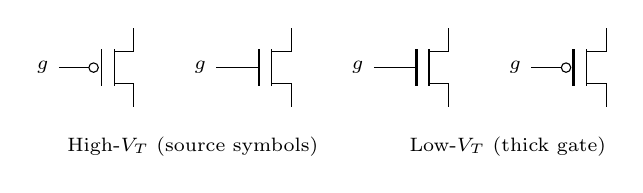
\begin{tikzpicture}[font=\scriptsize]
\mos{0}{1}{g}{1}\mos{2}{1}{g}{0}\node at(1,0){High-$V_T$ (source symbols)};
\mos{4}{1}{g}{0}\mos{6}{1}{g}{1}\foreach\x in{4,6}{\draw[line width=1.1pt](\x-.16,.77)--(\x-.16,1.23);}\node at(5,0){Low-$V_T$ (thick gate)};
\end{tikzpicture}\end{center}\begin{center}Figure 3: (a) CMOS circuit (b) original high-/low-$V_T$ symbols.\end{center}
\textbf{5. (10 points)} Three-dimensional (3D) integration technology using through-silicon via (TSV) is an emerging technology for integrated circuit (IC) designs. Figure 4 shows partial manufacturing steps for implementing a 3D IC using via-first and via-last TSV processes.
\begin{enumerate}[label=(\alph*),leftmargin=7mm]
\item List the correct manufacturing steps for via-first TSV process using the alphabet in sequence (hint: only three steps are needed). (5 points)
\item List the correct manufacturing steps for via-last TSV process using the alphabet in sequence (hint: only three steps are needed). (5 points)
\end{enumerate}
\begin{center}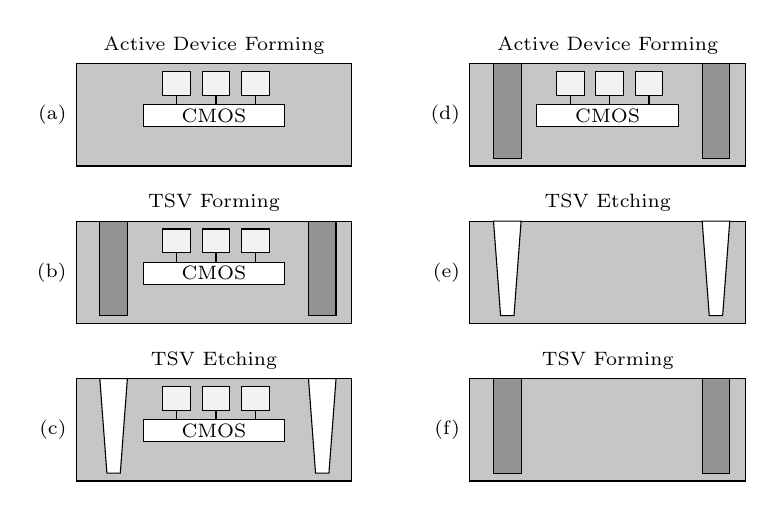
\begin{tikzpicture}[x=1cm,y=1cm,font=\scriptsize]
\foreach\x/\y/\a/\title/\active/\hole/\fillvia in{0/4/a/Active Device Forming/1/0/0,5/4/d/Active Device Forming/1/0/1,0/2/b/TSV Forming/1/0/1,5/2/e/TSV Etching/0/1/0,0/0/c/TSV Etching/1/1/0,5/0/f/TSV Forming/0/0/1}{
\begin{scope}[shift={(\x,\y)}]\draw[fill=gray!45](0,0)rectangle(3.5,1.3);\node[above]at(1.75,1.3){\title};\node[left]at(0,.65){(\a)};
\ifnum\active=1\draw[fill=white](.85,.5)rectangle(2.65,.78);\node at(1.75,.64){CMOS};\foreach\t in{1.1,1.6,2.1}{\draw[fill=gray!10](\t,.9)rectangle(\t+.35,1.2);\draw(\t+.175,.78)--(\t+.175,.9);}\fi
\ifnum\hole=1\foreach\t in{.3,2.95}{\draw[fill=white](\t,1.3)--(\t+.35,1.3)--(\t+.26,.1)--(\t+.09,.1)--cycle;}\fi
\ifnum\fillvia=1\foreach\t in{.3,2.95}{\draw[fill=gray!85](\t,.1)rectangle(\t+.35,1.3);}\fi
\end{scope}}
\end{tikzpicture}\\Figure 4: Partial manufacturing steps; schematic cross sections normalized.\end{center}
\newpage
\textbf{6. (15 points)} The figure shown below depicts a transistor-level schematic of the Boolean function Y.
\begin{enumerate}[label=(\alph*),leftmargin=7mm]
\item Show the corresponding gate-level schematic of the Boolean function Y. (5 points)
\item Assume that the resistances of the transistors P1, P2, P3, P4, P5, N1, N2, N3, N4 and N5 are $R_{P1},R_{P2},R_{P3},R_{P4},R_{P5},R_{N1},R_{N2},R_{N3},R_{N4},R_{N5}$, respectively. Also assume the parasitic capacitance of nodes 1, 2, 3 and 4 are $C_1,C_2,C_3,C_4$, respectively. Calculate the worst-case rise time and fall time of the circuit with a simple RC delay model. (10 points)
\end{enumerate}
\begin{center}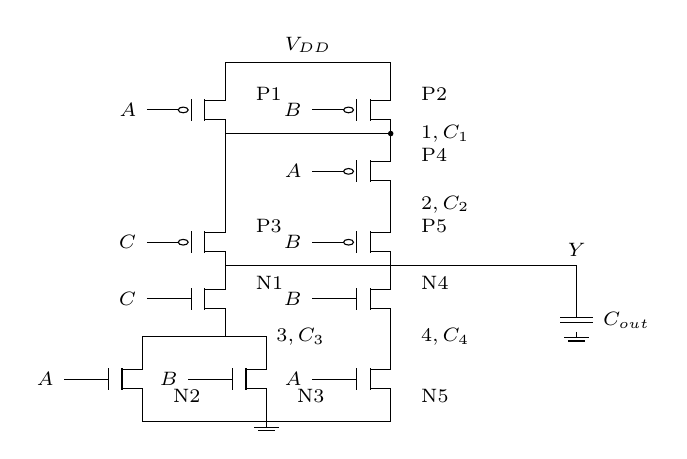
\begin{tikzpicture}[x=1.05cm,y=.6cm,font=\scriptsize]
\mos{1}{6}{A}{1}\mos{3}{6}{B}{1}\draw(1.25,6.5)--(1.25,7)--(3.25,7)--(3.25,6.5);\node[above]at(2.25,7){$V_{DD}$};\node[right]at(1.5,6.35){P1};\node[right]at(3.5,6.35){P2};
\draw(1.25,5.5)--(3.25,5.5);\fill(3.25,5.5)circle(1pt);\node[right]at(3.5,5.5){$1,C_1$};
\mos{3}{4.7}{A}{1}\draw(3.25,5.5)--(3.25,5.2);\node[right]at(3.5,5.05){P4};\draw(3.25,4.2)--(3.25,4);\node[right]at(3.5,4){$2,C_2$};
\mos{1}{3.2}{C}{1}\mos{3}{3.2}{B}{1}\draw(1.25,5.5)--(1.25,3.7);\draw(3.25,4)--(3.25,3.7);\node[right]at(1.5,3.5500000000000003){P3};\node[right]at(3.5,3.5500000000000003){P5};
\draw(1.25,2.7)--(3.25,2.7)--(5.5,2.7)node[above]{$Y$};\draw(5.5,2.7)--(5.5,1.6);\draw(5.3,1.6)--(5.7,1.6) (5.3,1.5)--(5.7,1.5);\grd{5.5}{1.3}\node[right]at(5.7,1.55){$C_{out}$};
\mos{1}{2}{C}{0}\mos{3}{2}{B}{0}\draw(1.25,2.7)--(1.25,2.5);\draw(3.25,2.7)--(3.25,2.5);\node[right]at(1.5,2.35){N1};\node[right]at(3.5,2.35){N4};
\draw(1.25,1.5)--(1.25,1.2)--(.25,1.2)--(.25,.8);\draw(1.25,1.2)--(1.75,1.2)--(1.75,.8);\node[right]at(1.75,1.2){$3,C_3$};\draw(3.25,1.5)--(3.25,.8);\node[right]at(3.5,1.2){$4,C_4$};
\mos{0}{.3}{A}{0}\mos{1.5}{.3}{B}{0}\mos{3}{.3}{A}{0}\node[right]at(.5,-0.04999999999999999){N2};\node[right]at(2,-0.04999999999999999){N3};\node[right]at(3.5,-0.04999999999999999){N5};
\draw(.25,-.2)--(.25,-.6)--(3.25,-.6)--(3.25,-.2);\draw(1.75,-.2)--(1.75,-.6);\grd{1.75}{-.6}
\end{tikzpicture}\end{center}\vfill\small This reconstruction provides editable question text and figures. All question text, named nodes, values and polarities are retained; geometry is normalized and handwritten annotations are omitted.\end{document}